%************************************************
\chapter{Decoding Pathology}\label{pathology}
%**************************************

\begin{startbox}{ConvNets diagnose pathology with good accuracy even from very short amounts of time} 
\item ConvNets reach around 85% accuracy
\item Can reach high accuracies using a single minute per recording during inference
\item Struggle with recordings where contextual features like age and sleep affect the doctors diagnosis
\item Seem to learn temporal slowing indicates pathology, strong occipital alpha indicates healthy
\end{startbox}


    We also evaluated our deep ConvNets for automatic medical diagnosis from
EEG. EEG is important in clinical practice both as a screening method as
well as for hypothesis-based diagnostics, e.g., in epilepsy or stroke.
One of the main limitations of using EEG for diagnostics is the required
time and specialized knowledge of experts that need to be well-trained
on EEG diagnostics to reach reliable results. Therefore, a deep-learning
approach that aids in the diagnostic process could make EEG diagnosis
more widely accessible, reduce time and effort for clinicians and
potentially make diagnoses more accurate. 

Text and figures in this
section are adapted from \citet{schirrmeisterdeeppathology}.
I was the main contributor to
\citet{schirrmeisterdeeppathology}.

\section{Dataset and Preprocessing}\label{dataset-and-preprocessing}

\subsection{Temple University Hospital EEG Abnormal
Corpus}\label{temple-university-hospital-eeg-abnormal-corpus}

\begin{table}[htb]
    \myfloatalign
    \begin{tabularx}{\textwidth}{p{0.15\textwidth}p{0.3\textwidth}p{0.2\textwidth}p{0.2\textwidth}}
    \toprule
        &
        &
        \tableheadlinewithwidth{0.2\textwidth}{Files} &
        \tableheadlinewithwidth{0.2\textwidth}{Patients} \\ 
        \midrule
    
        Train & Normal & 1379 (50\%) & 1238 (58\%) \\
        & Pathological & 1361(50\%) & 894 (42\%) \\
        & Rater Agreement & 2704 (99\%) & 2107 (97\%) \\
        & Rater Disagreement & 36 (1\%) & 25 (0\%) \\
        Evaluation & Normal & 150 (54\%) & 148 (58\%) \\
        & Pathological & 127 (46\%) & 105 (42\%) \\
        & Rater Agreement & 277 (100\%) & 253 (100\%) \\
        & Rater Disagreement & 0 (0\%) & 0 (0\%) \\
        \bottomrule
    \end{tabularx}
    \caption[TUH EEG Abnormal Corpus 1.1.2 Statistics]{
    \textbf{TUH EEG Abnormal Corpus 1.1.2 Statistics.} Obtained
from \url{https://www.isip.piconepress.com/projects/tuh_eeg/}. Rater
agreements refer to the agreement between the student annotator of the
file and the medical report written by a certified neurologist.
}
    \label{table-tuh-dataset}
\end{table}



    We used the Temple University Hospital (TUH) EEG Abnormal Corpus for
evaluating our deep ConvNets on pathology detection from EEG. The Temple
University Hospital (TUH) EEG Abnormal Corpus 1.1.2 is a dataset of
manually labeled normal and pathological clinical EEG recordings. It is
taken from the TUH EEG Data Corpus which contains over 16000 clinical
recordings of more than 10000 subjects from over 12 years
\citep{obeid\_temple\_2016}. The Abnormal Corpus contains
3017 recordings, 1529 of which were labeled normal and 1488 of which
were labeled pathological. The Corpus was split into a training and
evaluation set, see \Cref{table-tuh-dataset}. Recordings
were acquired from at least 21 standard electrode positions and with a
sampling rate of in most cases 250 Hz. Per recording, there are around
20 minutes of EEG data. The inter-rater agreement on between the medical
report of a certified neurologist and a medical student annotator was
99\% for the training recordings and 100\% for the evaluation
recordings, also see \Cref{table-tuh-dataset}.

\subsection{Preprocessing}\label{preprocessing}

    We minimally preprocessed the data with these steps: 1. Select a subset
of 21 electrodes present in all recordings. 2. Remove the first minute
of each recording as it contained stronger artifacts. 3. Use only up to
20 minutes of the remaining recording to speed up the computations. 4.
Clip the amplitude values to the range of $\pm800$ $\mu V$ to reduce
the effects of strong artifacts. 5. Resample the data to 100 Hz to
further speed up the computation.

\subsection{Decoding from Reduced EEG Time
Segments}\label{decoding-from-reduced-eeg-time-segments}

    We also evaluated the ConvNets on reduced versions of the datasets,
using only the first 1, 2, 4, 8, or 16 minutes after the first minute of
the recording (the first minute of the recordings was always excluded
because it appeared to be more prone to artifact contamination than the
later time windows). We reduced either only the training data, only the
test data, or both. These analyses were carried out to study how long
EEG recordings need to be for training and for predicting EEG
pathologies with good accuracies.

\section{Network Architectures}\label{network-architectures}

    We used our deep and shallow ConvNets with only minor modifications to
the architecture. To use larger time windows to make a single
prediction, we adapted the architectures by changing the final layer
kernel length so the ConvNets have an input length of about 600 input
samples, which correspond to 6 seconds for the 100 Hz EEG input.
Additionally, we moved the pooling strides of the deep ConvNet to the
convolutional layers directly before each pooling. This modification,
which we initially considered a mistake, allowed us to grow the ConvNet
input length without strongly increased computation times and provided
good accuracies in preliminary experiments on the training data;
therefore we decided to keep it.

\section{Network Training}\label{network-training}

    As in other studies, we optimized the ConvNet parameters using
stochastic gradient descent with the optimizer Adam
\cite{kingma\_adam:\_2014}. To make best use of the available
data, we trained the ConvNets on maximally overlapping time crops using
cropped training as described in \Cref{cropped-training}. Code
to reproduce the results of this study is available under
https://github.com/robintibor/auto-eeg-diagnosis-example.

\section{Automatic Architecture
Optimization}\label{automatic-architecture-optimization}

    We also carried out a preliminary study of automatic architecture
optimization to further improve our ConvNet architectures. To that end,
we used the automatic hyperparameter optimization algorithm SMAC
\citep{hutter\_sequential\_2011} to optimize architecture
hyperparameters of the deep and shallow ConvNets, such as filter
lengths, strides and types of nonlinearities. As the objective function
to optimize via SMAC, we used 10-fold cross-validation performance
obtained on the first 1500 recordings of the training data (using each
fold as an instance for SMAC to speed up the optimization). We set a
time limit of 3.5 hours for each configuration run on a single fold.
Runs that timed out or crashed (e.g., networks configurations that did
not fit in GPU memory) were scored with an accuracy of 0\%.

\section{Deep and Shallow ConvNets Reached State-of-the-Art
Results}\label{deep-and-shallow-convnets-reached-state-of-the-art-results}

\begin{table}[htb]
    \footnotesize
    \myfloatalign
    \begin{tabularx}{\textwidth}{p{0.2\textwidth}p{0.15\textwidth}p{0.15\textwidth}p{0.15\textwidth}p{0.15\textwidth}}
    \toprule
        &
        \tableheadlinewithwidth{0.15\textwidth}{Accuracy}&
        \tableheadlinewithwidth{0.15\textwidth}{Sensitivity} &
        \tableheadlinewithwidth{0.15\textwidth}{Specificity} &
        \tableheadlinewithwidth{0.15\textwidth}{Crop-accuracy} \\ 
        \midrule
    
Baseline \citep{abnormalLopez} & 78.8 & 75.4 & 81.9 & n.a. \\
Deep & 85.4 & 75.1 & 94.1 & 82.5 \\
Shallow & 84.5 & 77.3 & 90.5 & 81.7 \\
Linear & 51.4 & 20.9 & 77.3 & 50.2 \\
        \bottomrule
    \end{tabularx}
    \caption[TUH pathology decoding accuracies]{
\textbf{Decoding accuracies for discriminating normal and
pathological EEG with deep and shallow ConvNets.} For deep and shallow
ConvNets, mean over five independent runs with different random seeds.
Deep and shallow ConvNet outperformed the feature-based deep learning
baseline. Note that the baseline was evaluated on an older version of the corpus that has since been corrected to not contain the same patient in training and test recordings among other things. Results from \citet{schirrmeisterdeeppathology}.
}
\label{pathology-convnet-results}
\end{table}

    Both the deep and the shallow ConvNet outperformed the only results that
had been published on the TUH Abnormal EEG Corpus at the time (see
\Cref{pathology-convnet-results}). Both ConvNets were more
than 5\% better than the baseline method of a convolutional network that
included multiple fully connected layers at the end and took precomputed
EEG features of an entire recording as one input
\citep{abnormalLopez}.The ConvNets as applied here reduced
the error rate from about 21\% to about 15\%. We also tested a linear
classifier on the same 6-second inputs as our ConvNets. The linear
classifier did not reach accuracies substantially different from chance
(51.4\%).

    Interestingly, both of our ConvNet architectures already reached higher
accuracies than the baseline when evaluating single predictions from
6-second crops. The average per-crop accuracy of individual predictions
was only about 3\% lower than average per-recording accuracy (averaged
predictions of all crops in a recording). Furthermore, the individual
prediction accuracies were already about 3\% higher than the
per-recording accuracies of the baseline. This implies that predictions
with high accuracies can be made from just 6 seconds of EEG data.


\begin{figure}[htbp]
\myfloatalign
\subfloat[]{%
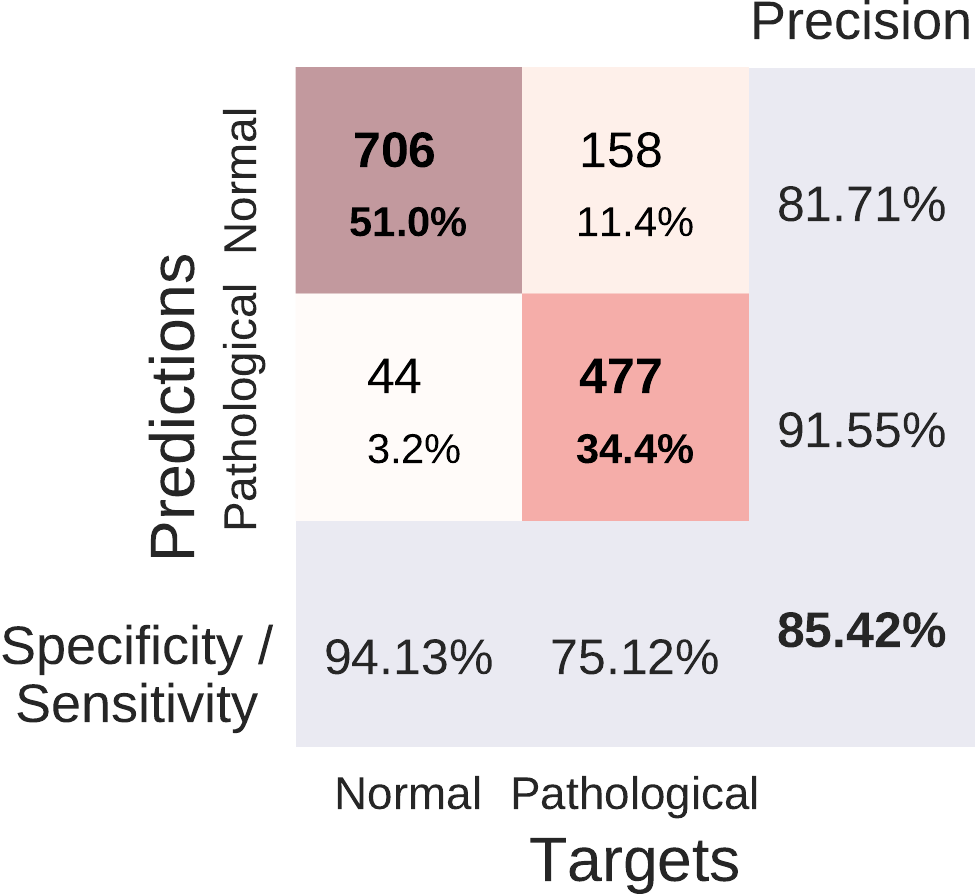
\includegraphics[width=0.408\linewidth]{images/ConfMatDeep.pdf-1.png}
}\hfill
\subfloat[]{%
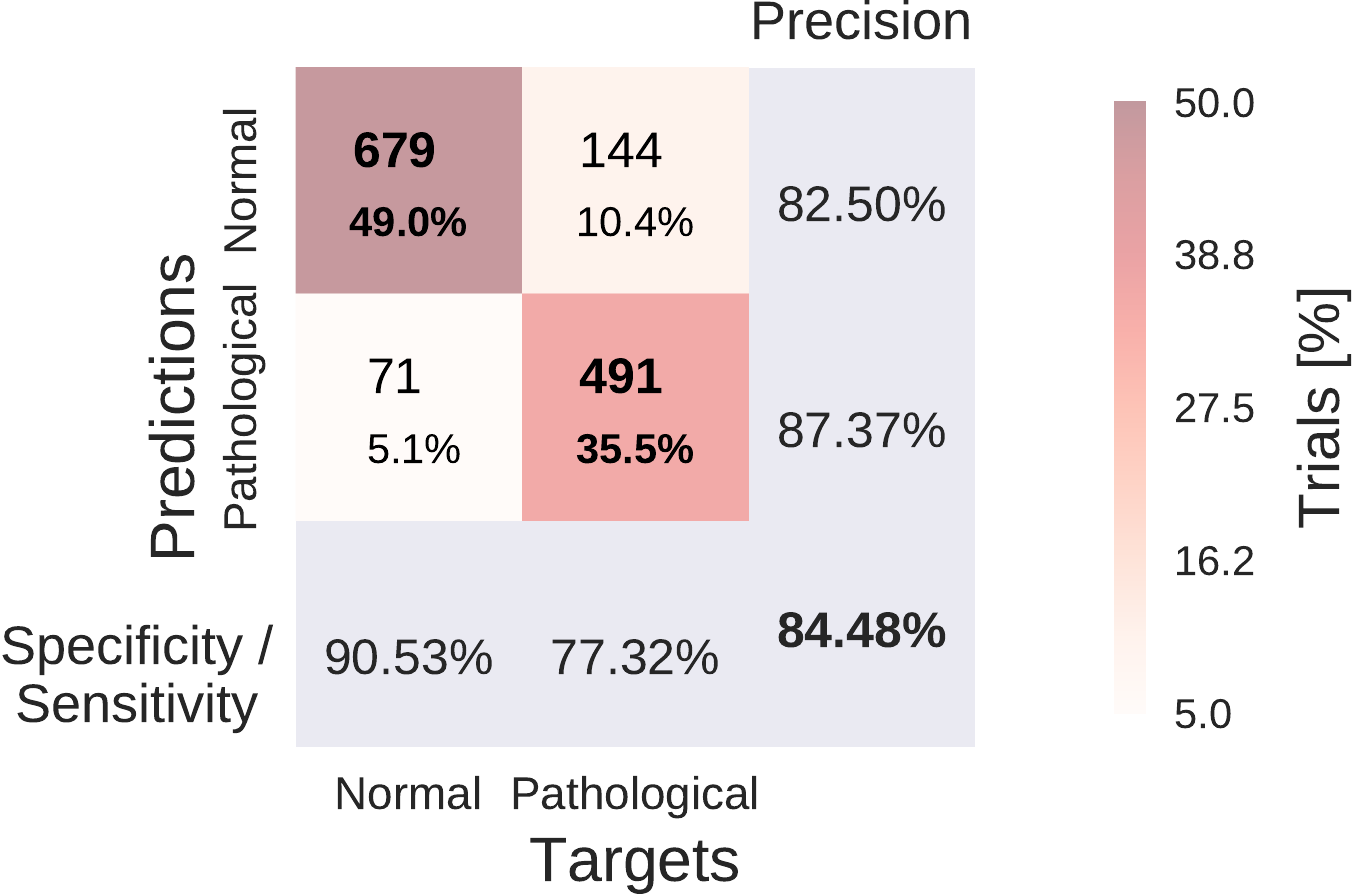
\includegraphics[width=0.562\linewidth]{images/ConfMatShallow.pdf-1.png}
}
\caption[Confusion Matrices for deep and shallow ConvNets]{\textbf{Confusion Matrices for deep and shallow ConvNets}, summed over five independent runs.
Each entry of row r and column c for upper-left 2x2-square: Number of trials of target r predicted as class c (also written in percent of all trials).
Bold diagonal corresponds to correctly predicted trials for both classes. Percentages and colors indicate fraction of trials in each cell relative to all trials.
The lower-right value: overall accuracy. The first two values in the bottom row correspond to sensitivity and specificity.
Rightmost column corresponds to precision defined as the number of trials correctly predicted for class r/number of trials predicted as class r. Figure from \citet{schirrmeisterdeeppathology}.}
\label{conf-mat-pathology-fig}
\end{figure}

    Both of our ConvNets made more errors on the pathological recordings, as
can be seen from \Cref{conf-mat-pathology-fig}. Both
ConvNets reached a specificity of above 90\% and a sensitivity of about
75-78\%. Confusion matrices between both approaches were very similar.
Relative to the baseline, they reached a similar sensitivity (0.3\%
smaller for the deep ConvNet, 1.9\% higher for the shallow ConvNet), and
a higher specificity (12.2\% higher for the deep ConvNet and 8.6\%
higher for the shallow ConvNet).

\begin{figure}[htbp]
\myfloatalign
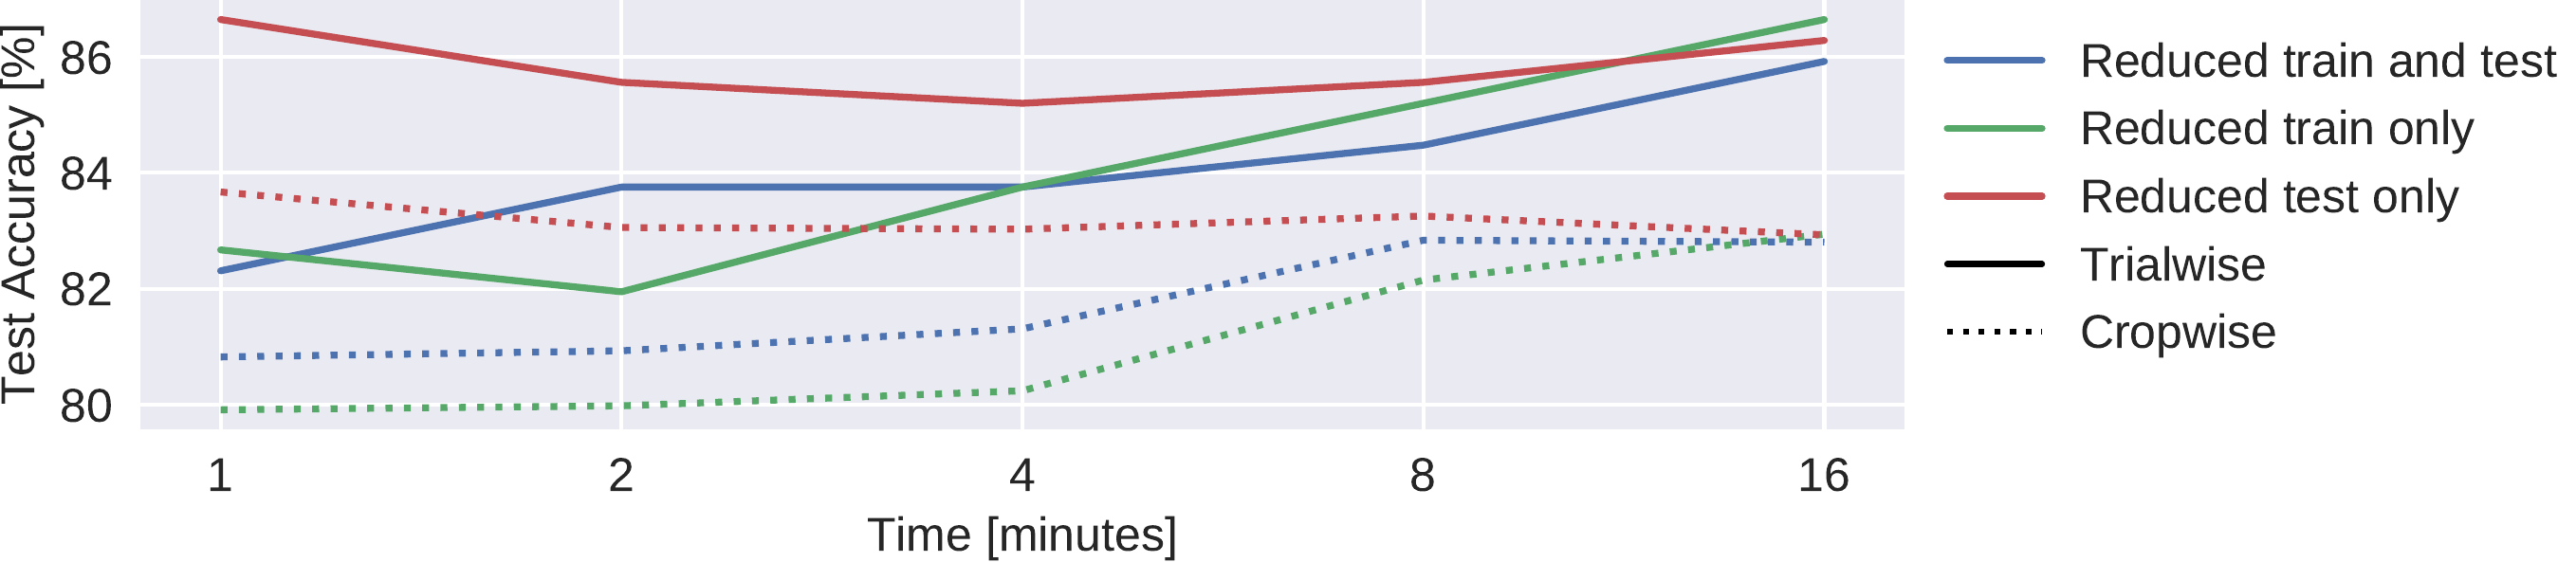
\includegraphics[width=\linewidth]{images/Time_Plot.pdf-1.png}
\caption[Results on reduced datasets for deep ConvNet]{\textbf{Results on reduced datasets for deep ConvNet.} Train and/or test (evaluation) dataset was reduced from 20 minutes per recording to 1,2,4,8, or 16 minutes per recording, results are shown on the test set. Notably, when only reducing the duration of the test set recordings, maximal accuracies were observed  when using just 1 minute. We note that these results are each based on one run only; the slightly better performance than in \Cref{pathology-convnet-results} may thus be due to noise. Figure from \citet{schirrmeisterdeeppathology}.}
\label{pathology-time-fig}
\end{figure}

\begin{figure}[htbp]
\myfloatalign
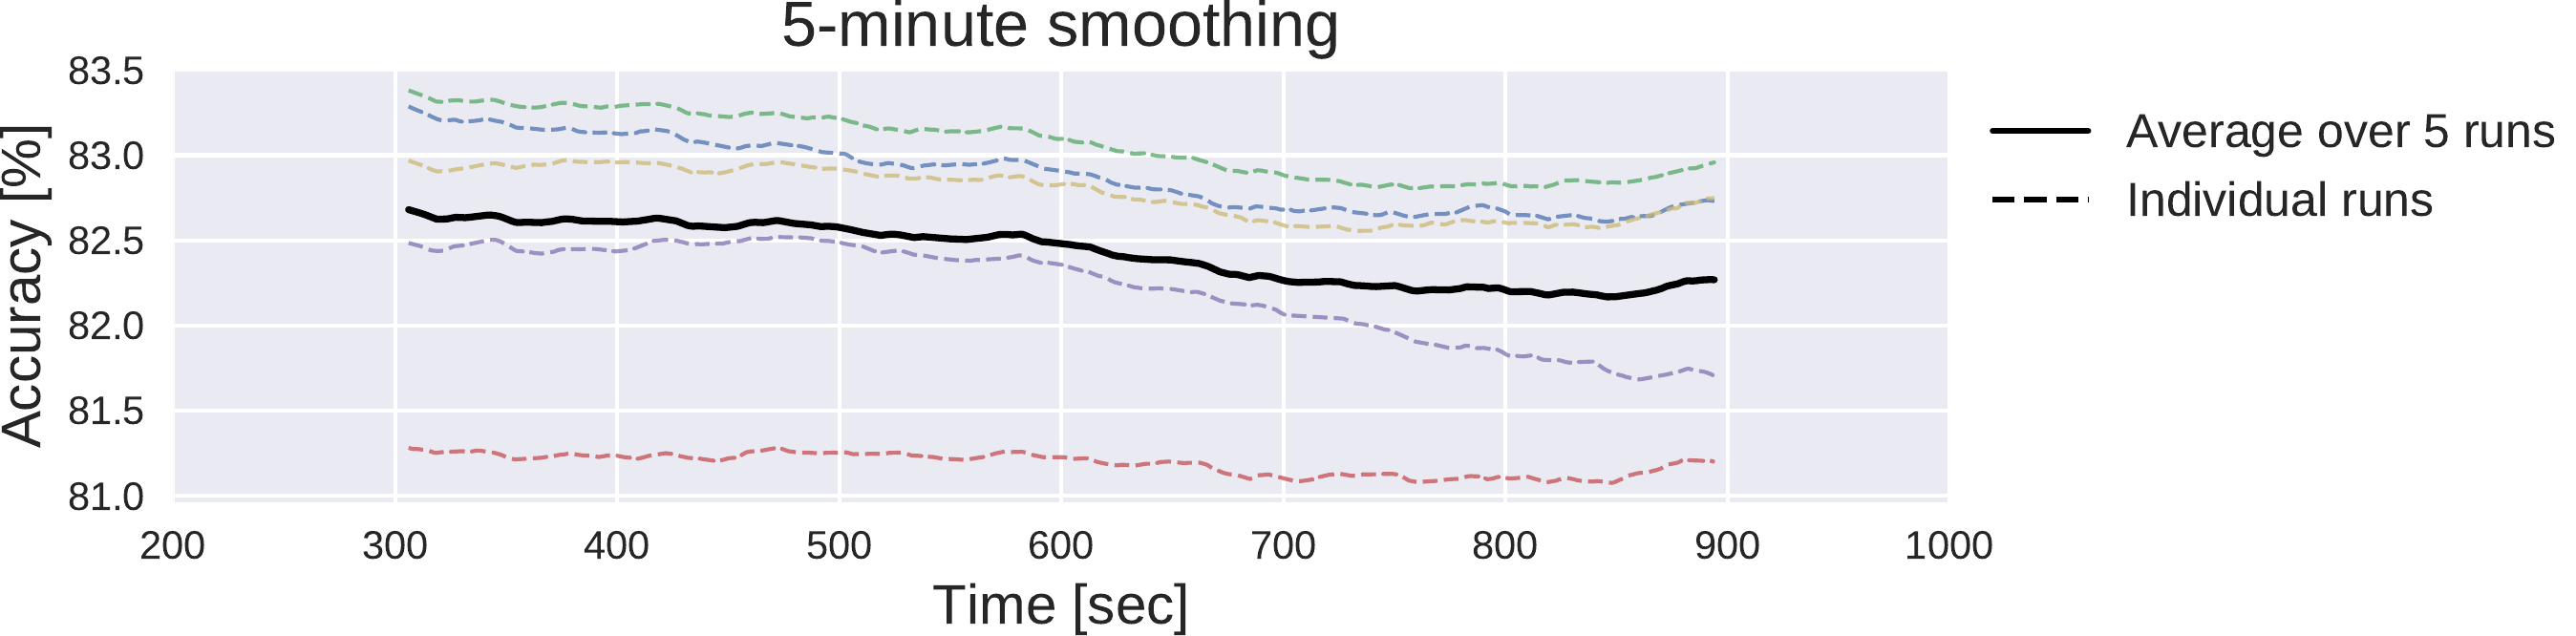
\includegraphics[width=\linewidth]{images/Time_Crop_Pred_Plot.pdf-1.png}
\caption[Moving average of cropwise accuracies for the deep ConvNet.]{\textbf{Moving average of cropwise accuracies for the deep ConvNet.}
5-minute moving averages of the cropwise accuracies of the deep ConvNet, averaged over all test set recordings.
Dashed lines represent 5 individual training runs with different random seeds, solid black line represents mean over results for these runs.
x-axis shows center of 5-minute averaging window.
Figure from \citet{schirrmeisterdeeppathology}.}
\label{time-crop-pred-fig}
\end{figure}

    Deep ConvNets already reached their best trialwise accuracies with only
one minute of data used for the prediction. While the reduction of the
amount of length of the training data led to crop- and trialwise
accuracy decreases on the test data, reductions in the test data did not
have such an effect (see \Cref{pathology-time-fig}).
Remarkably, both crop- and trialwise accuracies slightly decreased when
going from 1 minute to 2 or 4 minutes of test data. To investigate
whether earlier parts of the recordings might be more informative, we
also computed a 5-minute moving average of the cropwise accuracies on
the test data for the Deep ConvNet trained on the full data. We show the
average over all recordings for these moving averages in (see
\Cref{time-crop-pred-fig}). Noticeably, as expected,
accuracies slightly decreased with increasing recording time. However,
the decrease is below 0.5\% and thus should be interpreted cautiously.

\section{Architecture Optimization Yielded Unexpected New
Models}\label{architecture-optimization-yielded-unexpected-new-models}


\begin{figure}[htbp]
\myfloatalign
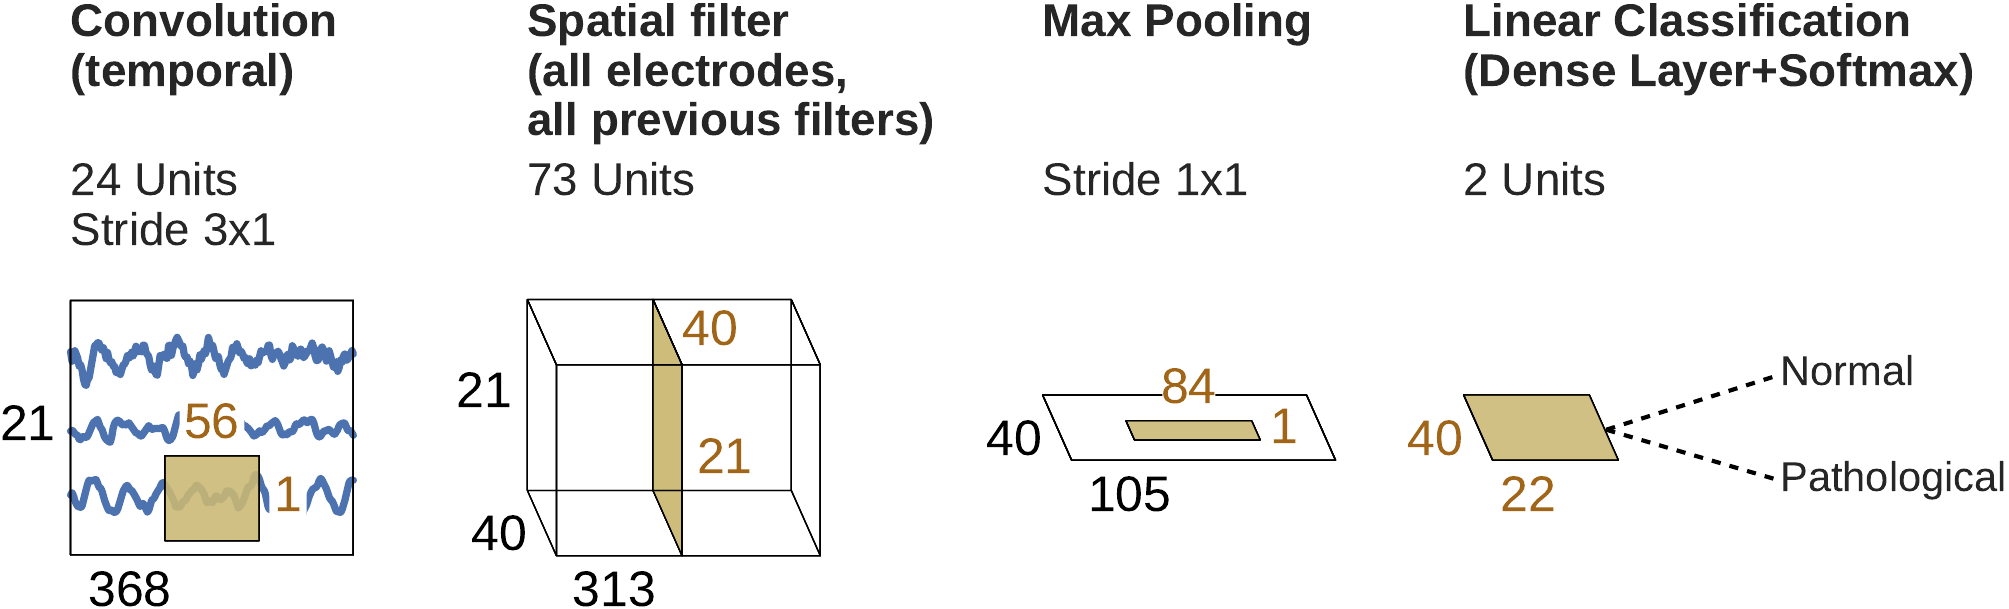
\includegraphics[width=\linewidth]{images/ShallowSmacNet.pdf-1.png}
\caption[Final shallow ConvNet architecture selected by SMAC]{\textbf{Final shallow ConvNet architecture selected by SMAC.}
Conventions as in Fig. \ref{fig:shallow-convnet}.
Note that max pooling is the only nonlinearity SMAC decided to use. Figure from \citet{schirrmeisterdeeppathology}.}
\label{pathology-smac-results}
\end{figure}


\begin{table}[htb]
    \myfloatalign
    \begin{tabularx}{\textwidth}{p{0.15\textwidth}p{0.25\textwidth}p{0.1\textwidth}p{0.1\textwidth}p{0.1\textwidth}p{0.1\textwidth}}
    \toprule
        &
        \tableheadlinewithwidth{0.25\textwidth}{Architecture configuration} &
        \tableheadlinewithwidth{0.1\textwidth}{Trial} &
        \tableheadlinewithwidth{0.1\textwidth}{Crop} &
        \tableheadlinewithwidth{0.1\textwidth}{Trial} &
        \tableheadlinewithwidth{0.1\textwidth}{Crop} \\ 
        \midrule
\textbf{Deep} & Default & 84.2 & 81.6 & 85.4 & 82.5 \\
& Optimized & 86.3 & 80.9 & 84.5 & 81.3 \\
\textbf{Shallow} & Default & 84.5 & 82.1 & 84.5 & 81.7 \\
& Optimized & 85.9 & 80.3 & 83.0 & 79.8 \\
        \bottomrule
    \end{tabularx}
    \caption[SMAC pathology decoding results]{
    \textbf{Decoding accuracies with the default of deep and
shallow ConvNets as well as versions optimized by automatic architecture
optimization.} Train here refers to 10-fold cross-validation on the 1500
chronologically earliest recordings of the training data.
. Results from \citet{schirrmeisterdeeppathology}.
}  \label{pathology-smac-results}
\end{table}

    The models discovered by automated architecture optimization were
markedly different from our original deep and shallow ConvNets. For
example, the optimized architectures used only 1.8 and 3.7 seconds of
EEG data for the optimized deep and shallow ConvNet, respectively, in
contrast to about 6 seconds in the original versions. While the improved
performance of these modified architectures for the 10-fold
cross-validation on the training dataset (2.1\% and 1.4\% improvement
for deep and shallow ConvNets, respectively) did not generalize to the
evaluation set (0.9\% and 1.5\% deterioration for deep and shallow
ConvNets, respectively, see \Cref{pathology-smac-results}),
the modifications to the original network architectures already provided
interesting insights for further exploration: For example, in the case
of the shallow ConvNet, the modified architecture did not use any of the
original nonlinearities, but used max pooling as the only nonlinearity
(see Fig. \Cref{shallow-smac-net-fig}), a configuration we
had not considered in our manual search so far.

    \hypertarget{visualization}{%
\section{Visualization}\label{visualization}}

    We analyzed the spectral power changes in the data itself and the
spectral characteristics of the function the deep networks learned on
the data.

    To understand class-specific spectral characteristics in the EEG
recordings, we analyzed band powers in five frequency ranges: delta
(0--4 Hz), theta (4--8 Hz), alpha (8--14 Hz), low beta (14--20 Hz), high
beta (20--30 Hz) and low gamma (30--50 Hz).

For this, we performed the following steps: 1. Compute a short-term
Fourier transformation with window size 12 seconds and overlap 6 seconds
using a Blackman-Harris window. 2. Compute the median over all band
powers of all windows and recordings in each frequency bin;
independently for pathological and normal recordings. 3. Compute the log
ratio of these median band powers of the pathological and normal
recordings. 4. Compute the mean log ratio over all frequency bins in
each desired frequency range for each electrode. 5. Visualize the
resulting log ratios as a topographical map.

To better understand the spectral characteristics of the function the
ConvNets learned used in this study, we also used the perturbation-based
visualization method described in
\citet{schirrmeisterdeephbm2017}.

\begin{figure*}[htbp]
\centering
\subfloat[Pathological vs. normal relative spectral bandpower differences for the training set. Shown is the logarithm of the ratio of the median bandpower of the pathological  vs. normal (according to the experts' ratings) EEG recordings.]{%
\label{bandpower-pathology-fig}
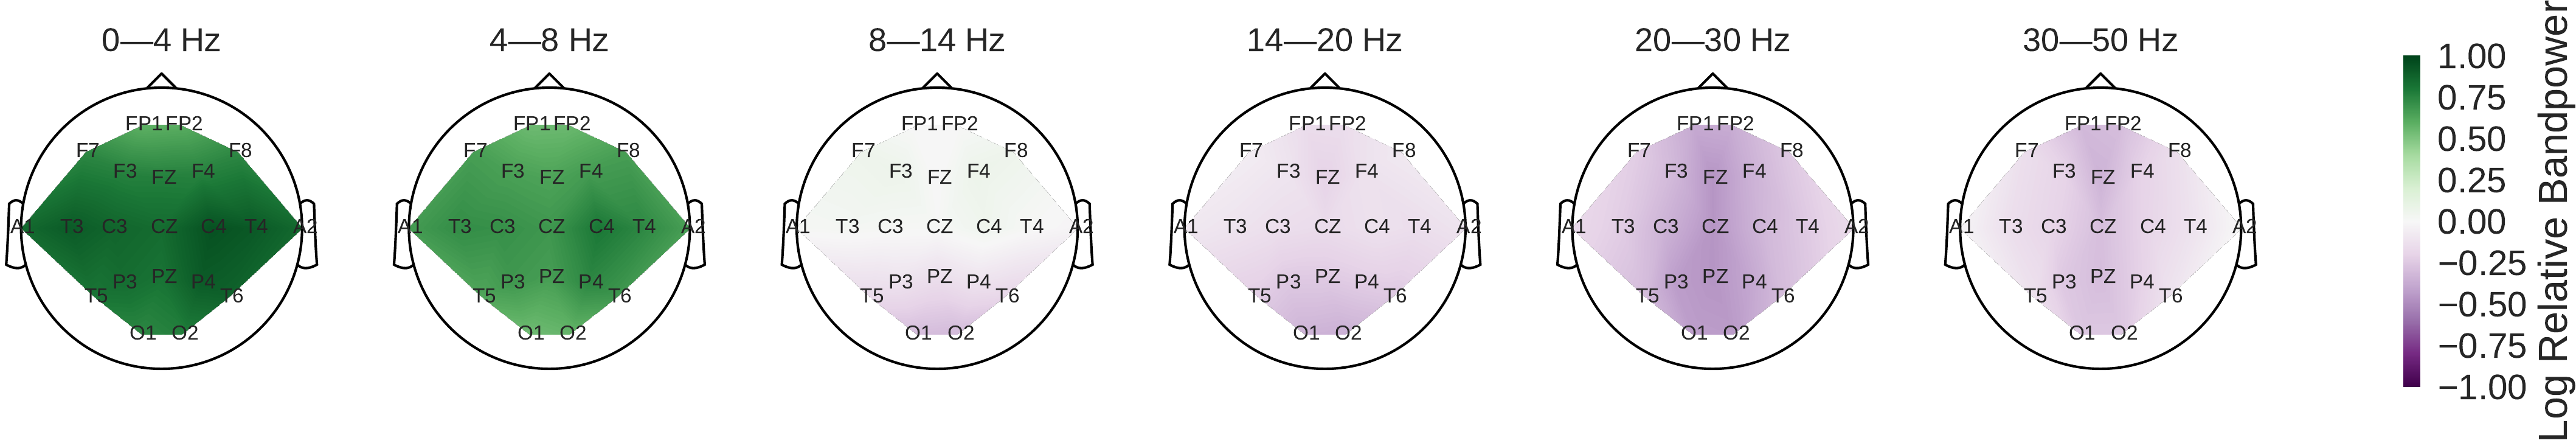
\includegraphics[width=0.8\textwidth]{images/Bandpower.pdf-1.png}
}
\vspace{0.4cm}

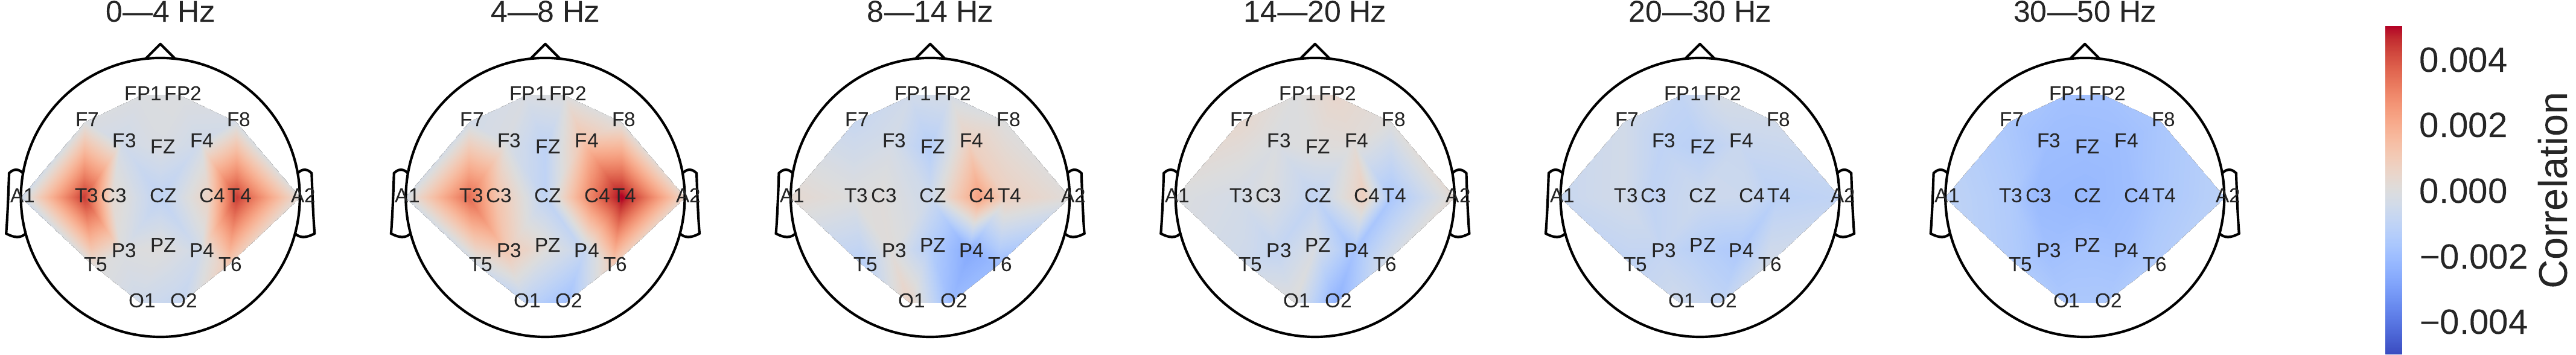
\includegraphics[width=0.8\textwidth]{images/PerturbationDeep.pdf-1.png}
\hfill
\subfloat[Input-perturbation network-prediction correlation maps for the deep (top) and shallow (bottom) ConvNet. Correlation of predictions for the pathological class with amplitude perturbations. Scalp maps revealed for example a bilateral positive correlation for the delta and theta frequency ranges and a spatially more broadly distributed negative correlation for the beta and low gamma frequency ranges, indicating that the ConvNets used these frequency components in their decisions
]{
\label{perturbation-network-pathology-fig}
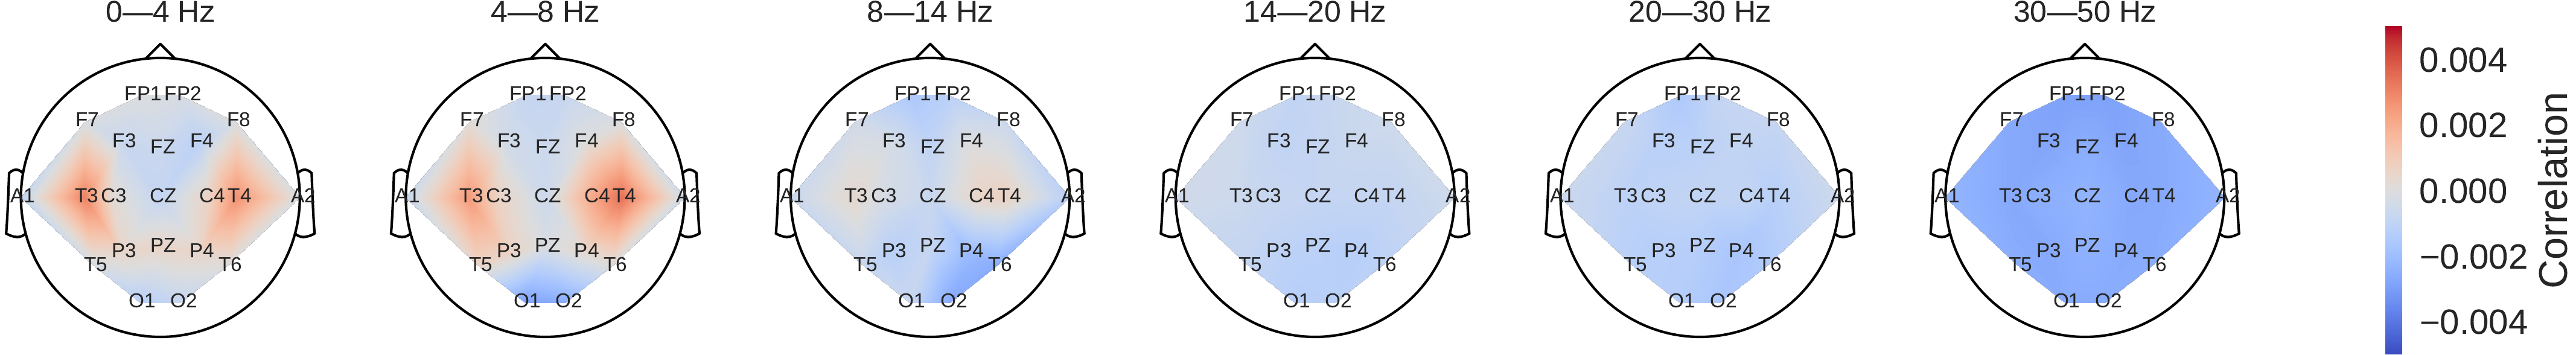
\includegraphics[width=0.8\textwidth]{images/PerturbationShallow.pdf-1.png}
}
\caption[Spectral power differences and input-perturbation network-prediction correlation maps]{\textbf{Spectral power differences and input-perturbation network-prediction correlation maps.} Figure from \citet{schirrmeisterdeeppathology}.}
\label{fig:visualization-results}
\end{figure*}

    Power was broadly increased for the the pathological class in the low
frequency bands (delta and theta range) and decreased in the beta and
low gamma ranges (\Cref{bandpower-pathology-fig}). Alpha
power was decreased for the occipital electrodes and increased for more
frontal electrodes.

    Scalp maps of the input-perturbation effects on predictions for the
pathological class for the different frequency bands showed effects
consistent with the power spectra in
(\Cref{perturbation-network-pathology-fig}). Both networks
strongly relied on the lower frequencies in the delta and theta
frequency range for their decoding decisions.

    \hypertarget{analysis-of-word-frequencies-in-the-medical-reports}{%
\section{Analysis of Word Frequencies in the Medical
Reports}\label{analysis-of-word-frequencies-in-the-medical-reports}}

    Furthermore, to better understand what kind of recordings are easier or
harder for the ConvNets to correctly decode, we analyzed the textual
clinical reports of each recording as included in the TUH Abnormal EEG
Corpus. Specifically, we investigated which words were relatively more
or less frequent in the incorrectly predicted recordings compared with
the correctly predicted recordings. We performed this analysis
independently for both the normal and the pathological class of
recordings. Concretely, for each class, we first computed the relative
frequencies $f_{i-}$ for each word $w_{i-}$ in the incorrectly
predicted recordings, i.e.:
$f_{i-} = \frac{|w_{i-}|}{\sum_{i}|w_{i-}|}$, where $|w_{i-}|$
denotes the number of occurrences for word $w_i$ in the incorrectly
predicted recordings. We then computed the frequencies $f_{i+}$ in the
same way and computed the ratios $r_i=f_{i-}/f_{i+}$. Finally, we
analyzed words with very large ratios ($\gg1$) and very small ratios
($\ll1$) by inspecting the contexts of their occurrences in the
clinical reports. This allowed us to gain insights into which
clinical/contextual aspects of the recordings correlated with ConvNets
failures.

Most notably, \texttt{small} and \texttt{amount} had a much larger word
frequency (15.5 times larger) in the incorrectly predicted pathological
recordings compared with the correctly predicted pathological
recordings. Closer inspection showed this is very sensible, as
\texttt{small\ amount} was often used to describe more subtle EEG
abnormalities (\texttt{small\ amount\ of\ temporal\ slowing},~
\texttt{Small\ amount\ of\ excess\ theta},~
\texttt{Small\ amount\ of\ background\ disorganization}, ~
\texttt{A\ small\ amount\ of\ rhythmic,} ~ \texttt{frontal\ slowing}), as this
subtlety of changes was likely the cause of the classification errors.

Secondly, other words with a notably different frequency were
\texttt{age} (9.7 times larger) and \texttt{sleep} (3 occurrences in 630
words of texts of incorrectly predicted recordings, not present in texts
of correctly predicted recordings). Both typically indicate the
clinician used the age of the subject or the fact that they were
(partially) asleep during the recording to interpret the EEG
(\texttt{Somewhat\ disorganized\ pattern\ for\ age},~
\texttt{Greater\ than\ anticipated\ disorganization\ for\ age.},~
\texttt{A\ single\ generalized\ discharge\ noted\ in\ stage\ II\ sleep.}).
Obviously, our ConvNets trained only on EEG do not have access to this
context information, leaving them at a disadvantage compared to the
clinicians and highlighting the potential of including contextual cues
such as age or vigilance in the training/decoding approach.

Inspection of the textual records of misclassified normal recordings did
not provide much insight, as they are typically very short (e.g.,
\texttt{Normal\ EEG.}, ~\texttt{Normal\ EEG\ in\ wakefulness.}).

Finally, consistent with the strong usage of the delta and theta
frequency range by the ConvNets as seen in the input-perturbation
network-prediction correlation maps
(\Cref{perturbation-network-pathology-fig}),
\texttt{slowing} and \texttt{temporal} are the 6th and 10th most
frequently occurring words in the textual reports of the pathological
recordings, while never occurring in the textual reports of the normal
recordings (irrespective of correct or incorrect predictions).

    \hypertarget{discussion}{%
\section{Discussion}\label{discussion}}

    To the best of our knowledge, the ConvNet architectures used in this
study achieved the best accuracies published so far on the TUH EEG
Abnormal Corpus. The architectures used were only very slightly modified
versions of ConvNet architectures that we previously introduced to
decode task-related information. This suggests that these architectures
might be broadly applicable both for physiological and clinical EEG. The
identification of all-round architectures would greatly simplify the
application of deep learning to EEG decoding problems and expand their
potential use cases.

Remarkably, the ConvNets already reached good accuracies based on very
limited time segments of the EEG recordings. Further accuracy
improvements could thus be possible with improved decoding models that
can extract and integrate additional information from longer timescales.
The exact nature of such models, as well as the amount of EEG they would
require, remains to be determined. More accurate decoding models could
either be ConvNets that are designed to intelligently use a larger input
length or recurrent neural networks, since these are known to inherently
work well for data with information both on shorter and longer term
scales. Furthermore, combinations between both approaches, for example
using a recurrent neural network on top of a ConvNet, as they have been
used in other domains like speech recognition
\cite{li_constructing_2015,sainath_convolutional_2015,sak_fast_2015},
are promising.

Our automated architecture optimization provided interesting insights by
yielding configurations that were markedly different from our
hand-engineered architectures, yet reached similar accuracies. Since the
marked improvements in training performance did not improve the
evaluation accuracies in this study, in future work, we plan to use more
training recordings in the optimization and study different
cross-validation methods to also improve evaluation accuracies. A
full-blown architecture search
\cite{mendoza_towards_2016,miikkulainen_evolving_2017,real_large-scale_2017, zoph_neural_2016,zoph_learning_2017}
could also further improve accuracy. With such improved methods it would
also be important not only to decode pathological vs.~normal EEG in a
binary fashion, but to also evaluate the possibility to derive more
fine-grained clinical information, such as the type of pathological
change (slowing, asymmetry, etc) or the likely underlying disorder (such
as epilepsy).

Any of these or other improvements might eventually bring the
machine-learning decoding performance of pathological EEG closer to
human-level performance. Since clinicians make their judgments from
patterns they see in the EEG and other available context information,
there is no clear reason why machine learning models with access to the
same information could not reach human-level accuracy. This human-level
performance is a benchmark for decoding accuracies that does not exist
for other brain-signal decoding tasks, e.g.~in decoding task-related
information for brain-computer interfaces, where there is inherent
uncertainty what information is even present in the EEG and no
human-level benchmark exists.

Our perturbation visualizations of the ConvNets' decoding behavior
showed that they used spectral power changes in the delta (0-4 Hz) and
theta (4-8 Hz) frequency range, particularly from temporal EEG channels,
possibly alongside other features
(\Cref{perturbation-shallow-pathology-fig}). This
observation is consistent both with the expectations implied by the
spectral analysis of the EEG data
(\Cref{bandpower-pathology-fig}) and by the textual reports
that frequently mentioned \texttt{temporal} and \texttt{slowing} with
respect to the pathological samples, but never in the normal ones. Our
perturbation visualization showed results that were consistent with
expectations that the ConvNets would use the bandpower differences
between the classes that were already visible in the spectra to perform
their decoding. Similarly, the textual reports also yielded plausible
insights, e.g., that \texttt{small\ amounts} of abnormalities as
indicated in the written clinical reports were more difficult for the
networks to decode correctly. Additionally, inspection of the textual
reports also emphasized the importance of integrating contextual
information such as the age of the subject.

Still, to yield more clinically useful insights and diagnosis
explanations, further improvements in ConvNet visualizations are needed.
Deep learning models that use an attention mechanism might be more
interpretable, since these models can highlight which parts of the
recording were most important for the decoding decision. Other deep
learning visualization methods like recent saliency map methods
\cite{kindermans_patternnet_2017,montavon_methods_2017}
to explain individual decisions or conditional generative adversarial
networks
\cite{mirza_conditional_2014,springenberg_unsupervised_2015}
to understand what makes a recording pathological or normal might
further improve the clinical benefit of deep learning methods that
decode pathological EEG.

Another option for more interpretable networks we explore in the next
chapter of this thesis are invertible networks, neural networks that are
designed to be invertible, see \Cref{invertible-networks} for
methods and \Cref{understanding-pathology} for results.

\begin{openbox}
\item How to further visualize the features networks learn to diagnose pathology?      
\end{openbox}
    
